\documentclass[conference]{IEEEtran}
\usepackage{cite}
\usepackage{amsmath,amssymb,amsfonts}
\usepackage{algorithmic}
\usepackage{graphicx}
\usepackage{textcomp}
\usepackage{xcolor}
\usepackage{tikz}
\usetikzlibrary{positioning}
\usepackage{minted}

\definecolor{myblue1}{RGB}{124,156,205}
\definecolor{myyellow1}{RGB}{202,217,126}

\def\BibTeX{{\rm B\kern-.05em{\sc i\kern-.025em b}\kern-.08em
    T\kern-.1667em\lower.7ex\hbox{E}\kern-.125emX}}
\begin{document}



\title{RustHDL - Rust as a Hardware Description Language}

\author{\IEEEauthorblockN{Samit Basu}
  Fremont, California
  USA
  basu.samit@gmail.com
}

\maketitle

\begin{abstract}
  RustHDL is an open source framework in which the Rust programming language is repurposed for 
  describing hardware.  It aims to bring the benefits of the Rust programming language to the 
  task of firmware design, and focuses on enabling the use
  of features such as strong typing, ease of design reuse, and rigorous safety and linting in
  the implementation of firmware.  RustHDL has a fairly extensive library of IP cores for 
  common hardware tasks, and has been fielded in commercial systems.  This paper describes the
  core concepts of RustHDL, and the lessons learned from the initial releases.
\end{abstract}

\begin{IEEEkeywords}
  Hardware description languages, Rust Programming Language, Field Programmable Gate Arrays,
  Design automation
\end{IEEEkeywords}


\section{Introduction}
There are a number of new hardware description languages (HDL) \cite{b1}-\cite{b5} that are being introduced that
attempt to remedy some of the shortcomings of the traditional Verilog or VHDL based workflow.
These HDLs tend to focus on newer features borrowed from the rapidly advancing fields of
software programming language design and compiler development.  Typically, these new HDLs
come with custom toolchains, new syntaxes and grammers, as well as new ways of thinking about
how hardware designs should best be expressed in text.

There is, however, an additional challenge that cannot be understated.  Hardware development
is typically quite difficult for those with traditional software engineering backgrounds.
The procedural, imperative mode of software development does not lend itself naturally to
the design of hardware systems.  As such, it is important to consider how "natural" an HDL
might feel to the developer using it.  As an example, MyHDL \cite{b3} is a Python-based HDL
that describes circuit function in terms of generators, which are functions that return
values over time.  The engineer is thus not exposed to the concepts of blocking and non-blocking 
assignments, priority assignments, etc.  Instead, the engineer writes fairly normal looking 
Python code, and the framework takes care of the translation to Verilog.

The use of a programming language as the basis for an HDL is not new.  However, modern programming
languages offer significant advantages over their predecessors.  The Rust programming 
includes a number of powerful features in a mainstream language such as:
\begin{itemize}
  \item Strong static typing
  \item Generic and const-generic programming
  \item Functional programming features
  \item A powerful package manager and ecosystem
  \item Built in test automation and documentation features
  \item High performance and multithreading
  \item A powerful macro system
\end{itemize}
These features lead the author to attempt to use the Rust programming language as the basis for
a hardware description language.  The goal was to leverage the power of the Rust programming language
to make the development of hardware designs easier, and to bring the benefits of the Rust programming
language to the task of hardware design.  The result of this effort is the open source RustHDL 
framework that allows for the development of firmware for Field Programmable Gate Arrays (FPGAs)
using the Rust programming language.  The framework has been used to develop commercial grade
firmware, and has been fielded in commercial products.  A large number of sample designs are
available on \verb|crates.io|, and the framework has seen some level of adoption by the open source
community.

The key components of both frameworks are:
\begin{itemize}
\item The use of the type system to allow for description of complex data without
  a synthesis overhead, and independent of the underlying toolchains support for
  types.
\item The use of composition and simple structs to describe hierarchies of design
  with encapsulation and the hiding of internal details.
\item The use of Rust itself as the programming language.  No new grammar is required
  and all of the infrastructure for supporting the Rust programming language, including training,
  compilers, linters, editors, etc. ``just work'' with RustHDL.  As a side effect,
  significant issues such as code sharing, documentation, and automated testing of hardware designs 
  are all handled by the Rust ecosystem.
\item The ability to integrate external IP cores and legacy designs (e.g., memory controllers,
  serializer/deserializers, PLLs, etc.) which cannot be described from first principles.
\item High performance simulation of hardware designs is built into the framework, so that
  testbenches and verification can be performed without the use of additional tools.
\end{itemize}

The organization of this paper is as follows.  Section~\ref{sec:related} describes related
works.  This is a particularly fruitful time for innovation in this space, and only a
sample of Rust-related projects are discussed. Section~\ref{sec:core} describes the 
basics of how Rust is used as an HDL using the RustHDL
framework.  This includes a discussion of how RustHDL leverages existing infrastructure 
for the Rust programming language to ease collaboration, testing, and sharing of hardware 
designs.  Section~\ref{sec:future} discusses the limitations observed from the initial
release of RustHDL, and the motivation for a rewrite.  Finally, Section~\ref{sec:conclusions}
presents conclusions.

\section{Background}\label{sec:related}

In considering the scope of background work, we will focus on the use of the Rust programming
language as primary in the consideration of Hardware Design Languages.  There are many modern
approaches to HDL in development (see \cite{b1} and the references therein for a good overview).  
From a high level, however, programming languages can influence HDLs in one of two ways:

\begin{itemize}
  \item Through grammar similarity.  A number of HDLs use syntaxes that are inspired or similar to
  programming languages in order to make the transition from software to hardware design easier.
  For example, Chisel \cite{b2} uses a Scala-like syntax, and Spade \cite{b1} uses a Rust-like syntax.
  The underlying implementation language is irrelevant (it happens to be Rust in the case of Spade).
  What is important is that the background experience and knowledge of the developer can be brought 
  to bear when understanding hardware descriptions if they use syntax and patterns from a broadly
  used programming language.
  \item As a host environment for the design.  In this case, a subset of the programming language (
    very similar in nature to a "synthesizable subset") is carved out of the broader programming language
    through some means, and then used to generate hardware designs within the context of the overall
    programming language.  An example here is MyHDL \cite{b3}, which uses Python as the host language, and 
    designs are expressed in a subset of Python that is synthesizable into Verilog.
\end{itemize}

While there are several examples of HDLs that use Rust as the inspiration language, RustHDL falls 
into the second category, and the author could find no other example like it.  In the 
first category, the most prominent examples are XLS \cite{b4} and Spade \cite{b1} and Veryl \cite{b5}.  
In all three of these cases, the language grammar and type system are inspired by Rust, but 
the actual tooling is separate from the Rust programming language and ecosystem.  In the case of 
\cite{b1, b5}, the relevant compilers are also written in Rust.  But XLS, which is quite close to 
Rust syntax, is written in C++.

RustHDL is unique in that \emph{hardware designs are expressed as valid Rust programs}.
This means that before a design can be synthesized, it must first pass the checks of the Rust
compiler, and be compiled into some form of working valid software program.
It also means that much of the infrastructure of the Rust programming language can be reused
by hardware designers.  Things like package management, documentation, test management and IDE 
integration all come for free.

\section{RustHDL Core Principles}\label{sec:core}

As this is not meant to be a tutorial, a very brief summary of the concepts used in RustHDL is presented
in order to orient the reader.  The core concepts of RustHDL are:

\begin{itemize}
  \item RustHDL is a subset of Rust.  As such all hardware designs must be valid Rust programs.  This includes
  all aspects of Rust validity checking including the borrow checker, type checking, initialization before 
  use, etc.
  \item Circuit elements are described architecturally as structs, and composition is used to combine 
  circuit elements into larger designs. Internal details of circuit elements can be exposed using the 
  \verb|pub| keyword, just as in a normal Rust struct.
  \item An \verb|update| function is used to describe the behavior of the circuit, and is roughly
  translated into Verilog using the macro extension capabilities of RPL.
  \item The system includes a reasonably high performance simulator with extensive tracing capabilities.
  This allows for the simulation of complex designs with a high degree of confidence, as well as 
  the use of RPL to write testbenches.
  \item Extensibility and collaboration are provided through the use of the Rust package manager \verb|cargo|, and 
  the ability to publish and share designs as crates on \verb|crates.io|.
\end{itemize}

While no one aspect of the above may be novel, the author believes that in combination, they present a 
novel and powerful way to describe hardware designs.  In the following subsections, each of these 
elements will be briefly touched upon and explained.  More thorough documentation is available on the
RustHDL website \cite{b6}.

\subsection{Circuit Elements}

Circuit elements in RustHDL are simply structs composed of other circuit elements.  The idea is to
provide effortless reuse and composition of circuit components.  Every circuit in RustHDL is composed
of three parts:
\begin{itemize}
  \item A struct that describes the architecture of the circuit.
  \item An \verb|update| function that describes signal propogation in the circuit internals.
  \item A constructor function that initializes the circuit.
\end{itemize}

As an example, the following from the RustHDL tutorial demonstrates a simple strobed blinker.  First, the
circuit element is defined as a struct, annotated with \verb|LogicBlock| to invoke the macro that generates
the necessary boilerplate required by the framework.

\begin{minted}[fontsize=\footnotesize]{rust}
use rust_hdl_core::prelude::*;
use crate::{dff::DFF, dff_setup};

/// A [Strobe] generates a periodic pulse train, 
/// with a single clock-cycle wide pulse
/// at the prescribed frequency.  The argument 
/// [N] of the generic [Strobe<N>] is used
/// to size the counter that stores the internal 
//  delay value.  
#[derive(Clone, Debug, LogicBlock)]
pub struct Strobe<const N: usize> {
    /// Set this to true to enable the pulse train.
    pub enable: Signal<In, Bit>,
    /// This is the strobing signal 
    /// it will fire for 1 clock cycle such that 
    /// the strobe frequency is generated.
    pub strobe: Signal<Out, Bit>,
    /// The clock that drives the [Strobe].  
    /// All signals are synchronous to this clock.
    pub clock: Signal<In, Clock>,
    threshold: Constant<Bits<N>>,
    counter: DFF<Bits<N>>,
}
\end{minted}

A couple of additional observations.  Signals have both a direction and a type.  The type of
signal can be any Rust type that implements the \verb|Synth| trait, and can include custom user
types and structs.  The \verb|derive| macro is used to generate the necessary boilerplate to make the 
\verb|Strobe| struct implement the \verb|Block| and \verb|Logic| traits.  The details of these implementations are
unimportant, and the user can simply use the \verb|Strobe| struct as if it were a normal Rust struct.  Also,
the D-type flip flop (DFF), which is critical to synchronous designs, is simply another circuit element that
is included in the internal structure of the \verb|Strobe| struct.  The RustHDL DFF is parameterized or 
generic over the type of data it holds, so in this case, it is holding an N-bit wide value.  The value of
\verb|N| is provided when the strobe is created.

Note also that the \verb|pub| keyword is used to expose parts of the circuit that are considered to be part
of it's public-facing interface.   The counter and threshold are internal implementation details and can be
changed without altering how this circuit is used in higher level designs.

The second part of the circuit encapsulates its behavior.  This is done by implementing the \verb|Logic| trait,
and requires only a single function, called \verb|update|.  The \verb|update| function describes the behavior
of the circuit via the propagation of signals through the internal structure of the circuit.  It is simply a Rust function
that must obey a few rules to ensure that the circuit can be synthesized.  Here is the \verb|update| function for
the \verb|Strobe| circuit:

\begin{minted}[fontsize=\footnotesize]{rust}
impl<const N: usize> Logic for Strobe<N> {
  #[hdl_gen]
  fn update(&mut self) {
    // Connect the counter clock to my clock
    // Also ensures that no latches are inferred
    // due to unassigned signals.
    dff_setup!(self, clock, counter);
    if self.enable.val() {
      self.counter.d.next = self.counter.q.val() + 1;
    }
    self.strobe.next = self.enable.val() & 
      (self.counter.q.val() == self.threshold.val());
    if self.strobe.val() {
      self.counter.d.next = 1.into();
    }
  }
}
\end{minted}

Here, the \verb|#[hdl_gen]| attribute is attached to the \verb|update| function to provide a way to convert the function
into Verilog.  The key thing to note, however, is that \emph{without this attribute, the function is still a valid Rust function}.
This means that the \verb|update| function can be tested, debugged, and run as a normal Rust function.  The \verb|#[hdl_gen]| adds
additional constraints to the code to ensure that it is synthesizable, but the Rust compiler still does the work of ensuring that the 
program input is valid.  This is in contrast to other Domain Specific Languages implemented in Rust (such as \cite{b10}) where the 
language only uses Rust's token structure, but the actual grammar and semantics are different.  In those cases, removing the 
macro attribute results in a non-compilable program.

The \verb|update| function follows a few rules that are laid out in the documentation.  In short:
\begin{itemize}
  \item Signals have two endpoints.  A \verb|.val()| endpoint that represents their current value, and a \verb|.next| endpoint that represents
    the value that the circuit is driving them to.
  \item Several (but not all) Rust flow control primitives are allowed, including \verb|match, if| \emph{statements} \
  and a very limited \verb|for|.  
  \item Local variables are allowed, but they must be declared in the architecture of the circuit, like any other element.
  These signals have a type of \verb|Local|, and are declared as \verb|my_sig: Signal<Local, T>|.  The types of any local 
  variables must be expressed as part of the struct declaration.  There is no type inference.
\end{itemize}

The last part of the circuit is the construction and initialization.  Here again, there is nothing special in RustHDL.  The 
constructor function is just a normal Rust function that populates the contents of the struct.  Because it can do anything
that a normal Rust function can do, arbitrary checks and computations (which are done prior to hardware synthesis) can be 
accomplished in the constructor.  For example, the constructor for the \verb|Strobe|, includes some checks that the 
desired strobe frequency will not overflow the size of the counter chosen for the design.  This is implemented as a set 
of assertions in the constructor and will fail at run time.  Making these checks compile-time is not currently possible on
stable Rust, but may be possible in the future \cite{b11}.

\subsection{Simulation and Testing}

One powerful aspect of RustHDL is the ease with which designs can be tested and simulated \emph{without} 
resorting to external tools.  Figure~\ref{fig:flow} illustrates some of the potential flow paths for a 
RustHDL design.  Without resorting to external tools or tooling, the RustHDL framework includes a high
performance event-based simulator that can be used to simulate the design, and generate traces of the circuit
signals.  These tests can lend a high degree of confidence in the correctness of the design before it is synthesized.

\begin{figure}[htbp]
  \centerline{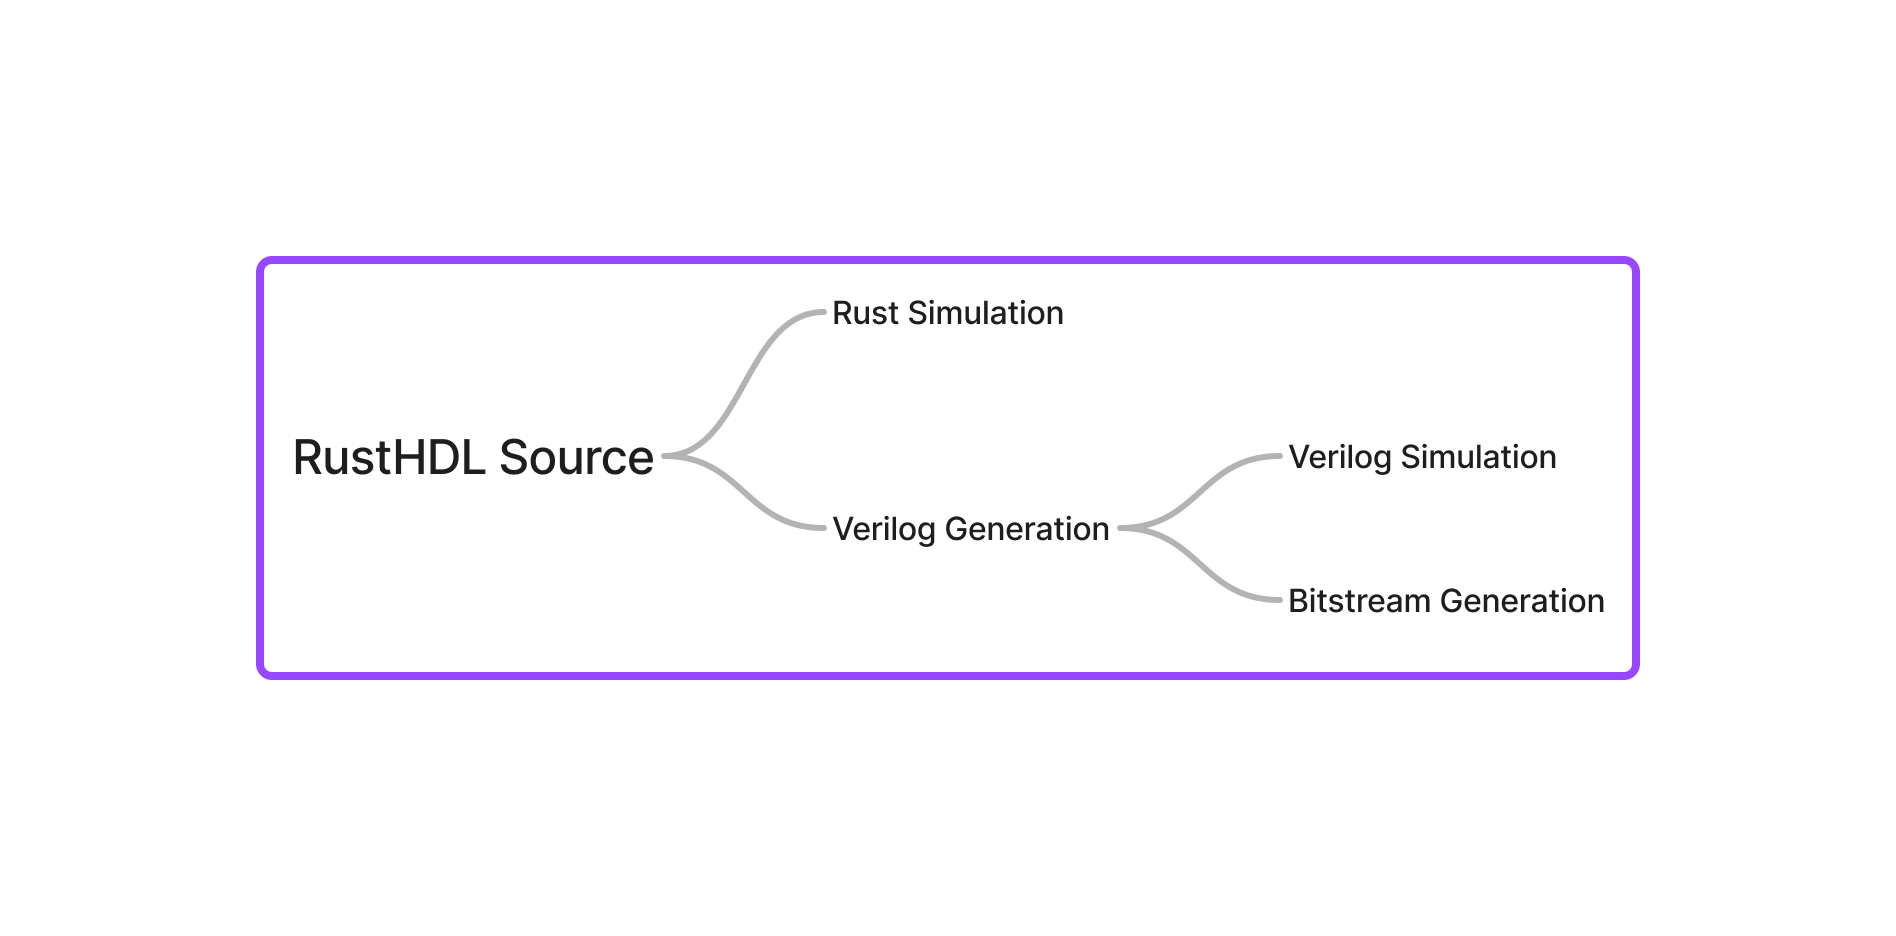
\includegraphics[width=10cm]{flow.png}}
  \caption{Flow of a RustHDL design}
  \label{fig:flow}
\end{figure}


As a result, RustHDL allows the engineer to write those testbenches using 
the full power of Rust.  The following example tests an SDRAM-backed FIFO implemented in RustHDL, that
includes a simulated SDRAM, and reads and writes random data to the FIFO concurrently with checks for
the integrity of the results.

\begin{minted}[fontsize=\footnotesize]{rust}
  #[test]
fn test_hls_sdram_fifo_works() {
  let mut uut = HLSSDRAMFIFOTest::default();
  let mut sim = Simulation::new();
  // v-- generate random data using Rust
  let data = (0..256)
      .map(|_| rand::thread_rng().gen::<u16>())
      .collect::<Vec<_>>();
  let data2 = data.clone();
  // v-- generate the clock
  sim.add_clock(4000, |x: &mut Box<_>| {
      x.clock.next = !x.clock.val()
  });
  // v-- this testbench feeds data to the fifo
  sim.add_testbench(move |mut sim: Sim<_>| {
      let mut x = sim.init()?;
      wait_clock_cycles!(sim, clock, x, 20);
      hls_fifo_write_lazy!(sim, clock, x, 
        fifo.bus_write, &data);
      sim.done(x)
  });
  // v-- this testbench drains data from the fifo
  //    and panics if it doesn't match the input
  sim.add_testbench(move |mut sim: Sim<_>| {
      let mut x = sim.init()?;
      wait_clock_cycles!(sim, clock, x, 20);
      hls_fifo_read_lazy!(sim, clock, x, 
        fifo.bus_read, &data2);
      sim.done(x)
  });
  // v-- both testbenches are run concurrently
  //    by the RustHDL event-based simulator
  sim.run_to_file(Box::new(uut), 200_000_000, 
      &vcd_path!("hls_sdram_fifo.vcd")).unwrap();
}
\end{minted}

The resulting trace file as shown in \ref{fig:trace} is quite complicated.  But the key is that
the testbench includes assertions to ensure correct behavior of the circuit, and will fail/panic 
if at any time the FIFO behaves incorrectly.  No manual visual inspection of the trace file is
required.  Indeed, it is far faster to run the simulation with no trace output at all, and simply 
have the testbenches encode the validity checks into their code. As such, the simulation can be run to 
verify the integrity of the design with a simple \verb|cargo test| command as part of a 
regular integration cycle.  Visual inspection of the trace output can be used when a test fails or
when debugging the circuit design.

\begin{figure*}[htbp]
  \centerline{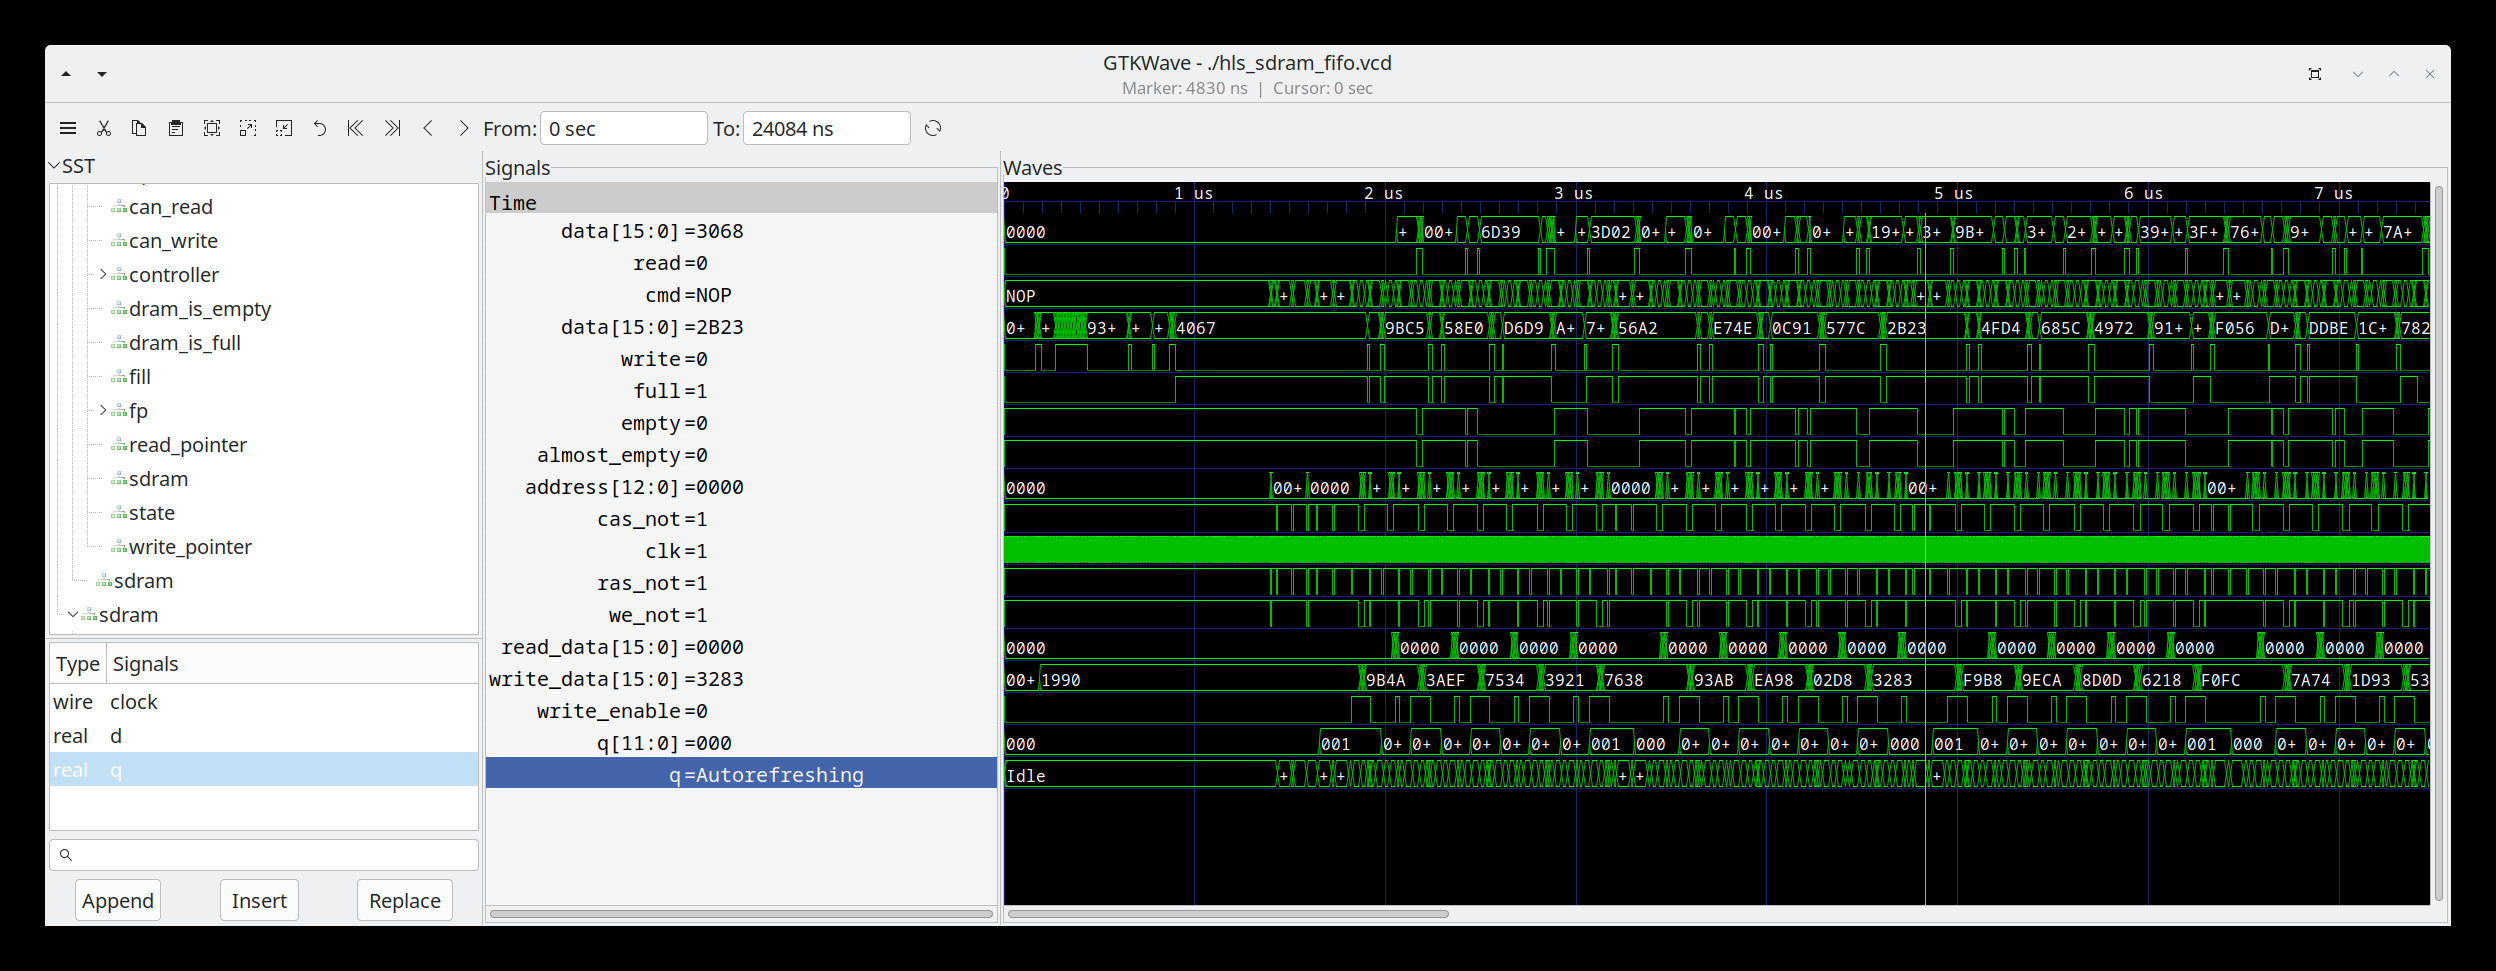
\includegraphics[width=18cm]{hls_sdram_fifo.png}}
  \caption{Sample simulation trace for the \textrm{HLSSDRAMFIFOTest} testbench}
  \label{fig:trace}
\end{figure*}
  
In the RustHDL test suite, a subset of the tests include a full synthesis, and are run on
actual FPGA boards attached to the host computer.  But these can be disabled if the necessary 
hardware and supporting software is missing.

\subsection{Synthesis and Extensibility}

Obviously, to get a RustHDL design onto an FPGA, it must be synthesized.  It is here that another 
advantage of the Rust ecosystem becomes apparent.  RustHDL includes the concept of a \emph{board support package} 
(a term borrowed from the embedded world), which is a software crate that provides the necessary infrastructure to
convert a RustHDL hardware design into a bitstream targeted at a specific device.  The BSP provides a function such 
as:

\begin{minted}[fontsize=\footnotesize]{rust}
  pub fn generate_bitstream<U: Block>
      (mut uut: U, prefix: &str) {}
\end{minted}

which takes a generic struct that implements a circuit, and converts it into a bitstream, using whatever tooling is
appropriate for the target device.  As noted in \cite{b1}, there is a significant challenge associated with using 
a standard programming language to express hardware designs - in particular, the range of acceptable expressions
must be limited to the common set from the destination language/HDL and the source language.  Without a full compiler,
the RustHDL grammar is limited to handle only those expressions that can be directly translated into Verilog.  
Concepts like early returns, and match expressions, which do not exist in Verilog, cannot be used in RustHDL.  

While the next version of RustHDL (RHDL) attempts to overcome these limitations, the benefit to such a close 
association between the two languages is that the generated Verilog is quite readable.  As one of the initial 
use cases for RustHDL was to generate IP cores that could be maintained in Verilog by other engineers, this feature
was critical.  To demonstrate, consider the following snippet of RustHDL:

\begin{minted}[fontsize=\footnotesize]{rust}
#[derive(LogicBlock)]
pub struct AlchitryCuPulser {
    pulser: Pulser,
    clock: Signal<In, Clock>,
    leds: Signal<Out, Bits<8>>,
}

impl Logic for AlchitryCuPulser {
    #[hdl_gen]
    fn update(&mut self) {
        self.pulser.enable.next = true;
        clock!(self, clock, pulser);
        self.leds.next = 0x00.into();
        if self.pulser.pulse.val() {
            self.leds.next = 0xAA.into();
        }
    }
}
\end{minted}

This simple blinker is translated into the following top level Verilog module:

\begin{minted}[fontsize=\footnotesize]{verilog}
module top(clock,leds);
  
  // Module arguments
  input wire  clock;
  output reg  [7:0] leds;
  
  // Stub signals
  reg  pulser$clock;
  reg  pulser$enable;
  wire  pulser$pulse;
  
  // Sub module instances
  top$pulser pulser(
      .clock(pulser$clock),
      .enable(pulser$enable),
      .pulse(pulser$pulse)
  );
  
  // Update code
  always @(*) begin
      pulser$enable = 1'b1;
      pulser$clock = clock;
      leds = 32'h0;
      if (pulser$pulse) begin
          leds = 32'haa;
      end
  end  
endmodule // top
\end{minted}

The relationship between the two is fairly evident, and one could theoretically maintain the Verilog
code without reference to the original RustHDL sources.

Based on experience, this close equivalence is primarily important when trying to understand and interpret 
the results of the toolchain while processing the design.  Issues that arise during timing analysis, or
during the place and route process are easier to map back into the RustHDL source code given the fairly 
close relationship between the two.  This issue will remain critical for all new HDL environments.  Because 
they ultimately rely upon existing toolchains, it can be difficult to interpret the results of those toolchains
in terms of the original HDL.

A key advantage of RustHDL is that this software module is completely decoupled
from the core library, and can be written and published by third parties (see \cite{b7} for an example of this in the wild).  
The core library can also be extended with new circuit elements (dubbed "widgets") that can be published on 
\verb|crates.io| and used by other engineers. As such one of the significant challenges in hardware design - 
that of sharing reusable components - is addressed by the Rust ecosystem.

The first class support that Rust provides for software package management also allows the core library to be extended
by others in the ecosystem.  Simply adding a package to the \verb|Cargo.toml| can enable new features such as 
easier wrapping of Verilog cores into RustHDL \cite{b8}.  Support for different use cases, such as ASICs, and different
FPGA families can be handled through external crates, avoiding the problems of a single point of coordination, testing
and publishing.

\section{Lessons Learned and the Path to RHDL}\label{sec:future}

RustHDL has been used to develop commercial grade firmware and is deployed in commercial products.  It has also seen 
some level of adoption by the open source community, with third party crates published on \verb|crates.io| that add board
support packages to RustHDL for different FPGAs, or augment the capabilities of the framework.  However, based on
feedback from users getting started with the framework, the following items became clear:

\begin{itemize}
  \item Engineers coming to a Rust-based HDL environment are likely to be familiar with the Rust programming language,
  and have grown accustomed to patterns and language features that are not supported by RustHDL.  For example, the 
  use of \verb|match| \emph{expressions}, and the use of complex types with their need to employ pattern matching to destructure 
  them are all idiomatic in Rust, but not supported by RustHDL.  This lack of support stems from the close 
  connection to Verilog of the generated code.
  \item Many idiomatic Rust patterns require some kind of support for Algebraic (Sum) Data Types (ADTs).  While RustHDL
  supports simple C-style enums, that is not sufficient to express many of the patterns common in Rust, including the 
  \verb|Result| and \verb|Option| patterns.
  \item The need to declare all local variables and their types up front is cumbersome.  Being able to freely rebind
  names and assign them is also critical to several standard Rust patterns (like shadowing).  This is also not
  possible in RustHDL.
  \item Function composition is not possible.  This makes the development of modular \emph{behavior} difficult.
  \item Testing is hard to grasp.  Testbenches are written in Rust, but require an understanding of the underlying
  event-based simulator that is used.  This makes testbenches difficult to write, and makes it difficult to use those
  testbenches in other environments (e.g., Verilog).
  \item Backends for multiple HDLs are needed including FIRTL, VHDL and others.  Some of those backends support
  rich type information to be carried on signals, and so would benefit from propagating that typed information through
  to the HDL instead of simply generating bit vectors.
\end{itemize}

After taking all of these considerations into account, a new framework, named RHDL was planned that addressed these issues.  The 
core differences between RustHDL and RHDL are:

\begin{itemize}
  \item Full support for Rust data types, including ADTs, tuples, etc.
  \item Full support of Rust syntax inside functions (with the exception of pointers), which includes 
  match and if \emph{expressions}, early returns, etc.
  \item Full support for function composition.
  \item Support for local variables/rebindings, as well as pattern matching in \verb|match| expressions.
  \item The use of a function iterator-style description of testbenches in which testbenches are written in 
  straight Rust, and consumed by the simulator (so that the details of how the circuit is simulated can be ignored).
  \item Support for thorough analysis of the design, including identification of potential timing issues, as well as
  metastability detection, and clock domain crossings.
  \item Support for multiple backend languages is possible, even for those that want type information.
\end{itemize}

These items required a signficantly broader scope and far more effort on the compiler side of the framework.  In particular,
the first four items require the development of a full compiler that works alongside \verb|rustc| to process the source. 
This embedded compiler performs the following passes, each of which is necessary to achieve the full support of Rust:
\begin {itemize}
  \item Type inference to add support for local rebindings and pattern matching.
  \item Lowering of Rust expressions to an intermediate representation (which is a kind of RTL-SSA assembly code).  This
  step is where early returns, if expressions and pattern matching are lowered to ROM tables and muxes.
  \item Optimization passes to remove unneeded registers, and unreachable code.
  \item Validation passes that ensure there are no latches generated, and that all types are preserved through the lowering.
  \item Analysis passes that look for potential timing issues, and metastability.
  \item Linking of translation units into a single design.  This is where support for function composition and black boxes is
  provided.
  \item Generation of Verilog (or whatever target HDL is desired - Verilog only at this time).
\end{itemize}
Apart from the analysis passes, the remainder of the compiler is implemented and working.  The analysis passes are still in
development.  As mentioned in Section~\ref{sec:core}, one significant challenge is maintaining coherence between the analysis 
results reported by the synthesis tools and the RHDL source code.  This is a significant challenge and still an area of 
active research and experimentation.


\section{Conclusions}\label{sec:conclusions}

Rust is an excellent language to serve as the basis of building powerful environments for 
hardware design.  RustHDL demonstrates how the compiler, tooling, infrastructure and 
community of the Rust programming language can be leveraged to build a robust and 
collaborative environment for hardware design.  The initial release and use of RustHDL,
along with the feedback provided by the open source community lead to a roadmap for 
the successor of RustHDL (RHDL), which employs additional software technology to bring
the full expressiveness of the underlying language to hardware design.  The author believes
that the use of Rust as a basis for hardware design is a powerful and compelling idea, and
that the RHDL project will be a significant step forward in the development of hardware
design environments.

\begin{thebibliography}{00}
\bibitem{b1} Spade.
\bibitem{b2} Chisel
\bibitem{b3} MyHDL
\bibitem{b4} XLS
\bibitem{b5} Veryl
\bibitem{b9} Rust Programming Language
\bibitem{b6} RustHDL
\bibitem{b7} bsp
\bibitem{b8} macro
\bibitem{b10} DIESL
\bibitem{b11} const generic computation
\end{thebibliography}
\vspace{12pt}

\end{document}
